
% case name
\chapter{waq3d~aed2~flume}
%
% - Purpose & Description:
%     These first two parts give reader short details about the test case,
%     the physical phenomena involved, the geometry and specify how the numerical solution will be validated
%
\section{Purpose}
%
This test shows the coupling between \telemac{3d} and the water quality library AED2. It checks if AED2 coupling is working well when water is flowing.
%
\section{Description}
%
A simple channel is considered, the same as canal example (500~m long, 100~m wide).\\
The hydrodynamic parametrization is exactly the same as canal example.
%
\subsection{Geometry and Mesh}
%
%
\subsubsection{Bathymetry}
%
Flat horizontal bottom
%
\subsubsection{Geometry}
%
Channel length = 500~m\\
Channel width = 100~m
%
\subsubsection{Mesh}
%
551 triangular elements\\
319 nodes\\
10 levels regularly spaced on the vertical.
%
%
\subsection{Physical parameters}
Horizontal constant viscosity: no  \\
Vertical turbulence model: Nezu and Nakagawa mixing length model\\
Wind: no\\
Bottom friction : Strickler law with coefficient 50m$^{1/3}$s$^{-1}$
%
%
\subsection{Water quality parameters}
Coupling with Waqtel and Water quality processes = 6 (AED2)
aed2.nml file contains the AED2 parametrization. The following modules are activated :
\begin{itemize}
	\item sedflux
	\item oxygen
	\item carbon
	\item silica
	\item nitrogen
	\item phosphorus
	\item organic matter
	\item phytoplankton
	\item tracer
	\item total
\end{itemize}
It is the same water quality parametrization as waq3d\_aed2 test case.
%
\subsection{Initial and Boundary Conditions}
%
\subsubsection{Initial conditions}
%
Steady flow (previous result file)\\
Initial concentrations are homogeneous\\
%
\subsubsection{Boundary conditions}
%
Upstream prescribed flow rate: 50~m$^3$/s\\
Downstream prescribed elevation: 0.5~m\\
Constant concentrations\\

%
\subsection{General parameters}
%
Time step: 1~s\\
Simulation duration: 40~s
%

\subsection{Numerical parameters}
%
hydrostatic version\\
%

%
\subsection{Comments}
Among the tracers, only the temperature, the oxygen, methan, silica and phytoplankton concentrations are printed in the result files.

% - Results:
%     We comment in this part the numerical results against the reference ones,
%     giving understanding keys and making assumptions when necessary.
%
%
\section{Results}

As an example the Figure~\ref{fig:res} shows the õxygen and phytoplankton concentrations at the end of the calculation.
%

\begin{figure} [H]
\centering
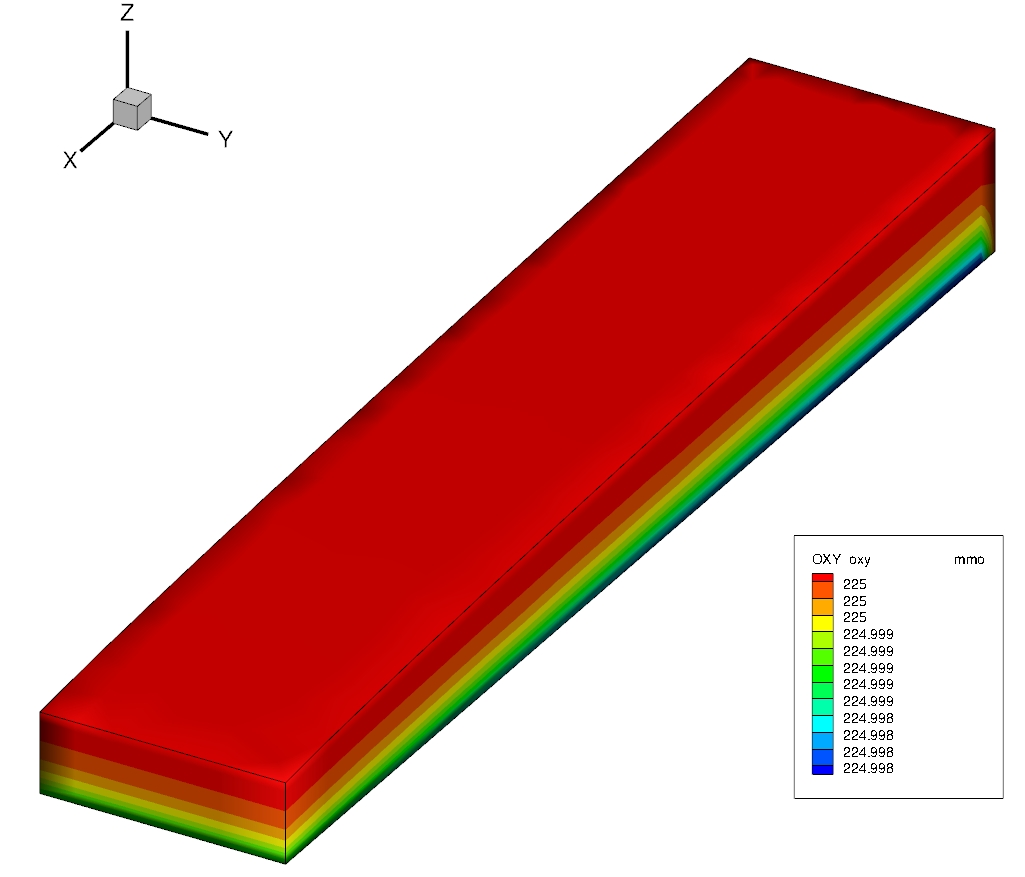
\includegraphics[scale=0.3]{flume_oxy.jpg}
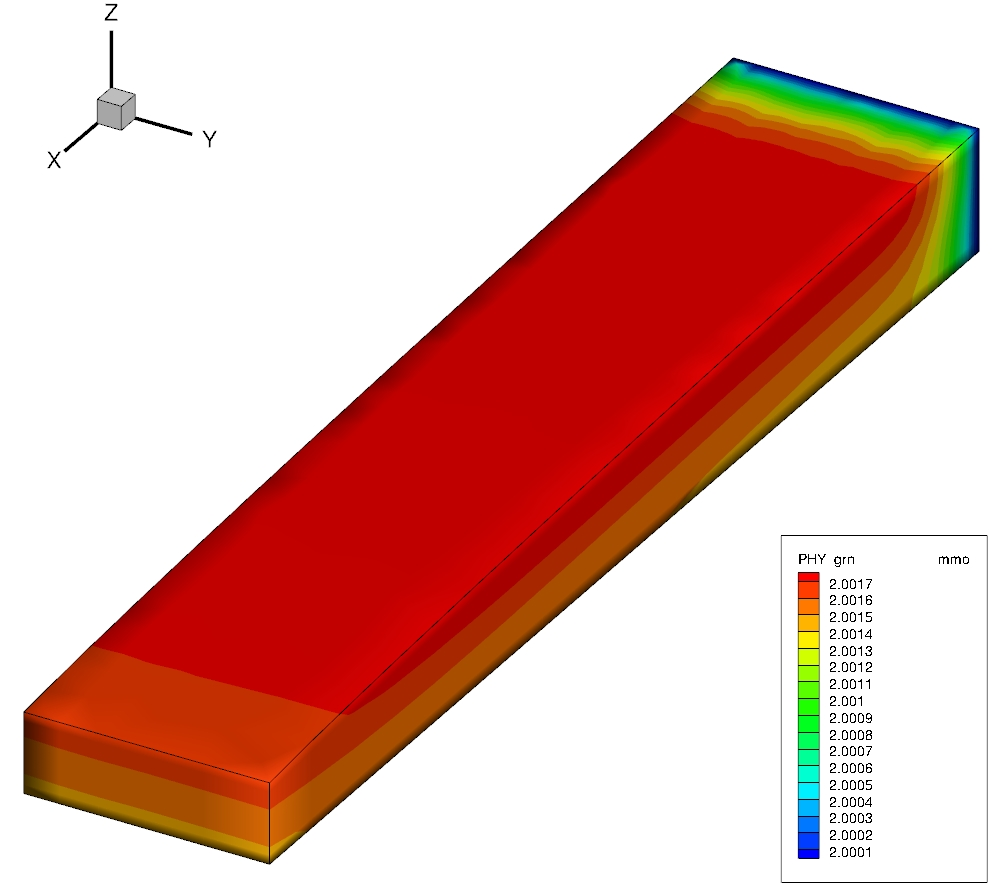
\includegraphics[scale=0.3]{flume_phyto.jpg}
 \caption{waq3d aed2 flume test: oxygen and phytoplankton concentrations after 40s.}
 \label{fig:res}
\end{figure}


%
\section{Conclusion}
%
\telemac{3d} is coupled with AED2
%
% Here is an example of how to include the graph generated by validateTELEMAC.py
% They should be in test_case/img
%\begin{figure} [!h]
%\centering
%\includegraphics[scale=0.3]{../img/mygraph.png}
% \caption{mycaption}\label{mylabel}
%\end{figure}
%
% bibliography
%\section{Reference}

